\documentclass{article}

% Language setting
% Replace `english' with e.g. `spanish' to change the document language
\usepackage[english]{babel}

% Set page size and margins
% Replace `letterpaper' with `a4paper' for UK/EU standard size
\usepackage[letterpaper,top=2cm,bottom=2cm,left=3cm,right=3cm,marginparwidth=1.75cm]{geometry}

% Useful packages
\usepackage{multicol}
\usepackage{ragged2e}
\usepackage{amssymb}
\usepackage{amsmath}
\usepackage{graphicx}
\usepackage[framemethod=tikz]{mdframed}
\usepackage{array}
\usepackage{blindtext}
\usepackage{mathtools}
\numberwithin{equation}{subsection}
\numberwithin{figure}{subsection}
%\usepackage[paperwidth=10cm]{geometry}
\usepackage{tkz-euclide}
%\usepackage{tikz}
\usepackage{enumitem}
\usepackage{listings}
\usetikzlibrary{
  circuits.logic,
  circuits.logic.US,
  positioning
}

\usepackage[colorlinks=true, allcolors=blue]{hyperref}

\providecommand{\mbf}{\mathbf}
\newcommand{\myvec}[1]{\ensuremath{\begin{pmatrix}#1\end{pmatrix}}}
\providecommand{\qfunc}[1]{\ensuremath{Q\left(#1\right)}}
\providecommand{\cbrak}[1]{\ensuremath{\left\{#1\right\}}}
\providecommand{\brak}[1]{\ensuremath{\left(#1\right)}}
\providecommand{\lsbrak}[1]{\ensuremath{{}\left[#1\right.}}
\providecommand{\rsbrak}[1]{\ensuremath{{}\left.#1\right]}}
\providecommand{\rcbrak}[1]{\ensuremath{\left.#1\right\}}}
\providecommand{\lcbrak}[1]{\ensuremath{\left\{#1\right.}}
\providecommand{\sbrak}[1]{\ensuremath{{}\left[#1\right]}}
\providecommand{\pr}[1]{\ensuremath{\Pr\left(#1\right)}}
\providecommand{\system}{\overset{\mathcal{H}}{ \longleftrightarrow}}
\providecommand{\abs}[1]{\left\vert#1\right\vert}
\providecommand{\dec}[2]{\ensuremath{\overset{#1}{\underset{#2}{\gtrless}}}}
\providecommand{\gauss}[2]{\mathcal{N}\ensuremath{\left(#1,#2\right)}}
\newcommand{\solution}{\noindent \textbf{Solution: }}
%\renewcommand{\thefigure}{\theproblem}
\renewcommand\thesection{\arabic{section}}
\renewcommand\thesubsection{\thesection.\arabic{subsection}}
\renewcommand\thesubsubsection{\thesubsection.\arabic{subsubsection}}
\renewcommand{\thefigure}{\arabic{subsection}.\arabic{figure}}
\renewcommand{\theequation}{\arabic{section}.\theenumi.\arabic{equation}}
\renewcommand{\thefigure}{\theenumi}
%\renewcommand{\labelenumi}{\thesubsection.\arabic{enumii}}
\title{Digital Communication Assignment}
\author{Anusha Jella}
\begin{document}
\maketitle
\tableofcontents
\section{Axioms}
\begin{enumerate}%[label=\thechapter.\arabic*,ref=\thechapter.\theenumi]
\item A and B are events such that $\pr A=0.42, \pr B=0.48$ and $\pr {\text{A and B}}=0.16$. \\
Determine 
\begin{enumerate}
\item $\pr{\text{not A}}$ 
\item $\pr{\text{not B}}$  
\item $\pr{\text{A or B}}$ 
\end{enumerate}
\solution
\begin{enumerate}
\item $\pr{\text{not A}}$
\begin{align}
\pr{A^{\prime}} &= 1 - \pr A \\
&= 1 - 0.42 \\
&= 0.58 
\end{align}

\item $\pr{\text{not B}}$
\begin{align}
\pr{B^{\prime}} &= 1 - \pr B \\
&= 1 - 0.48 \\
&= 0.52
\end{align}

\item $\pr{\text{A or B}}$
\begin{align}
\pr{\text{A+B}} &= \pr A + \pr B - \pr {AB} \\
&= 0.42 + 0.48 - 0.16 \\
&= 0.74
\end{align}
\end{enumerate}
\item Given that the events A and B are such that $P(A)=\frac{1}{2}, P(A + B)=\frac{3}{5}$ and $P(B)=p$. Find $p$ if they are 
\begin{enumerate}
\item mutually exclusive
\item independent\\
\solution
\begin{enumerate}
	\item 
		In this case
\begin{align}
\pr{A + B} &=\pr{A} + \pr{B}&
\\
\implies \frac{3}{5}&=\frac{1}{2}+p&
\\
\therefore  p &= \frac{1}{10}&
\end{align}
\item 
Given A and B are independent events,
then,

\begin{align}
\pr{A + B} &=\pr{A} + \pr{B} - \pr{A B}& 
\\
\implies \pr{A + B} &=\pr{A} + \pr{B} - \pr{A}\pr{B}&
\\
\implies \frac{3}{5}&=\frac{1}{2}+ p - \frac{p}{2}&
\\
\therefore p &= \frac{1}{5}&
\end{align}
\end{enumerate}
\end{enumerate}
\end{enumerate}
\section{Conditional Probability}
\begin{enumerate}%[label=\thechapter.\arabic*,ref=\thechapter.\theenumi]
\item 
Given that E and F are events such that $P(E)=0.6, P(F)=0.3$ and $P(E F)=0.2$, find $P(E \mid F)$ and $P(F \mid E)$.
\\
\solution
\begin{align}
\pr{E|F}=&\frac{\pr{E  F}}{\pr{F}}=\frac{0.2}{0.3}=\frac{2}{3}&  
\\
\pr{F|E}=&\frac{\pr{E  F}}{\pr{E}}=\frac{0.2}{0.6}=\frac{1}{3}&  
\end{align}
	\item Compute $\pr{A|B}$, if $\pr{B}=0.5$ and $\pr{AB}=0.32$. 
		\\
\solution
By using property of conditional probability we have,
\begin{align}
\pr{A|B}=\frac{\pr{AB}}{\Pr{B}}=\frac{0.32}{0.5}=0.64
\end{align}
\end{enumerate}
\section{Two Dice}
\subsection{Sum of Independent Random Variables}
Two dice, one blue and one grey, are thrown at the same time.   The event defined by the sum of the two numbers appearing on the top of the dice can have 11 possible outcomes 2, 3, 4, 5, 6, 7, 8, 9, 10, 11 and 12.  A student argues that each of these outcomes has a probability $\frac{1}{11}$.  Do you agree with this argument?  Justify your answer.
\begin{enumerate}[label=\thesubsection.\arabic*.,ref=\thesubsection.\arabic{figure}]
%\numberwithin{equation}{enumi}
%\numberwithin{figure}{enumi}
\item {\em The Uniform distribution} Let $X_i \in \cbrak{1,2,3,4,5,6}, i = 1,2,$ be the random variables representing the outcome for each die.  Assuming the dice to be fair, the probability mass function (pmf) is expressed as 
\begin{align}
\label{eq:dice_pmf_xi}
p_{X_i}(n) = \pr{X_i = n} =
\begin{cases}
\frac{1}{6} & 1 \le n \le 6
\\
0 & otherwise
\end{cases}
\end{align}
The desired outcome is
\begin{align}
\label{eq:dice_xdef}
X &= X_1 + X_2,
\\
\implies X &\in \cbrak{1,2,\dots,12}
\end{align}
The objective is to show that
\begin{align}
p_X(n) \ne \frac{1}{11}
\label{eq:dice_wrong}
\end{align}
\begin{flushleft}
 \textsc{solution:} the following python code is available for proof.
 \end{flushleft}
 \begin{center}
\fbox{\parbox{10.5cm}{\href{https://github.com/AnushaJella/FWC1/blob/main/Digital-communications/codes/chapter3/dice_1.py}{/codes/chapter3/dice$\_$1.py}}}
\end{center}
\item {\em Convolution: }
From \eqref{eq:dice_xdef},
\begin{align}
p_X(n) &= \pr{X_1 + X_2 = n} = \pr{X_1  = n -X_2}
\\
&= \sum_{k}^{}\pr{X_1  = n -k | X_2 = k}p_{X_2}(k)
\label{eq:dice_x_sum}
\end{align}
after unconditioning.  $\because X_1$ and $X_2$ are independent,
\begin{multline}
\pr{X_1  = n -k | X_2 = k} 
\\
= \pr{X_1  = n -k} = p_{X_1}(n-k)
\label{eq:dice_x1_indep}
\end{multline}
From \eqref{eq:dice_x_sum} and \eqref{eq:dice_x1_indep},
\begin{align}
p_X(n) = \sum_{k}^{}p_{X_1}(n-k)p_{X_2}(k) = p_{X_1}(n)*p_{X_2}(n)
\label{eq:dice_x_conv}
\end{align}
where $*$ denotes the convolution operation. 
%\cite{proakis_dsp}.  
Substituting from \eqref{eq:dice_pmf_xi}
in \eqref{eq:dice_x_conv},
\begin{align}
p_X(n) = \frac{1}{6}\sum_{k=1}^{6}p_{X_1}(n-k)= \frac{1}{6}\sum_{k=n-6}^{n-1}p_{X_1}(k)
\label{eq:dice_x_conv_x1}
\end{align}
\begin{align}
\because p_{X_1}(k) &= 0, \quad k \le 1, k \ge 6.
\end{align}
From \eqref{eq:dice_x_conv_x1},
%
\begin{align}
p_X(n) &= 
\begin{cases}
0 & n < 1
\\
\frac{1}{6}\sum_{k=1}^{n-1}p_{X_1}(k) &  1 \le n-1 \le  6
\\
\frac{1}{6}\sum_{k=n-6}^{6}p_{X_1}(k) & 1 < n-6 \le 6
\\
0 & n > 12
\end{cases}
\label{eq:dice_x_conv_cond}
\end{align}
Substituting from \eqref{eq:dice_pmf_xi} in \eqref{eq:dice_x_conv_cond},
\begin{align}
p_X(n) &= 
\begin{cases}
0 & n < 1
\\
\frac{n-1}{36} &  2 \le n \le  7
\\
\frac{13-n}{36} & 7 < n \le 12
\\
0 & n > 12
\end{cases}
\label{eq:dice_x_conv_final}
\end{align}
satisfying \eqref{eq:dice_wrong}.
\begin{flushleft}
 \textsc{solution:} the following python code is available for proof.
 \end{flushleft}
 \begin{center}
\fbox{\parbox{10.5cm}{\href{https://github.com/AnushaJella/FWC1/blob/main/Digital-communications/codes/chapter3/1_2_dice_conv.py}{/codes/chapter3/1$\_$2$\_$dice$\_$conv.py}}}
\end{center}
\item {\em The $Z$-transform: }
The $Z$-transform of $p_X(n)$ is defined as 
%\cite{proakis_dsp}
\begin{align}
P_X(z) = \sum_{n = -\infty}^{\infty}p_X(n)z^{-n}, \quad z \in \mathbb{C}
\label{eq:dice_xz}
\end{align}
%
From \eqref{eq:dice_pmf_xi} and \eqref{eq:dice_xz}, 
\begin{align}
P_{X_1}(z) =P_{X_2}(z) &= \frac{1}{6}\sum_{n = 1}^{6}z^{-n}
\\
&=\frac{z^{-1}\brak{1-z^{-6}}}{6\brak{1-z^{-1}}},  \abs{z} >1
\label{eq:dice_xiz}
\end{align}
upon summing up the geometric progression.  
\begin{align}
\because p_X(n) &= p_{X_1}(n)*p_{X_2}(n),
\\
P_X(z) &= P_{X_1}(z)P_{X_2}(z)
\label{eq:dice_xzprod_def}
\end{align}
The above property follows from Fourier analysis and is fundamental to signal processing. 
%\cite{proakis_dsp}. 
From \eqref{eq:dice_xiz} and \eqref{eq:dice_xzprod_def},
\begin{align}
P_X(z) &= \cbrak{\frac{z^{-1}\brak{1-z^{-6}}}{6\brak{1-z^{-1}}}}^2
\\
&= \frac{1}{36}\frac{z^{-2}\brak{1-2z^{-6}+z^{-12}}}{\brak{1-z^{-1}}^2}
\label{eq:dice_xzprod}
\end{align}
Using the fact that 
%\cite{proakis_dsp}
\begin{align}
p_X(n-k) &\system{Z}P_X(z)z^{-k},
\\
nu(n)&\system{Z} \frac{z^{-1}}{\brak{1-z^{-1}}^2}
\end{align}
after some algebra, it can be shown that
%{\tiny
\begin{multline}
\frac{1}{36}\lsbrak{\brak{n-1}u(n-1) - 2 \brak{n-7}u(n-7)}
\\
\rsbrak{ +\brak{n-13}u(n-13)}
\\
\system{Z}
\frac{1}{36}\frac{z^{-2}\brak{1-2z^{-6}+z^{-12}}}{\brak{1-z^{-1}}^2}
\label{eq:dice_xz_closed}
\end{multline}
%}
where 
\begin{align}
u(n) =
\begin{cases}
1 & n \ge 0
\\
0 & n < 0
\end{cases}
\end{align}
From \eqref{eq:dice_xz}, \eqref{eq:dice_xzprod} and \eqref{eq:dice_xz_closed}
\begin{multline}
p_{X}(n) = \frac{1}{36}\lsbrak{\brak{n-1}u(n-1) 
}
\\
\rsbrak{- 2 \brak{n-7}u(n-7)+\brak{n-13}u(n-13)}
\end{multline}
which is the same as \eqref{eq:dice_x_conv_final}.  Note that  \eqref{eq:dice_x_conv_final} can be obtained from \eqref{eq:dice_xz_closed} using contour integration as well.
% \cite{proakis_dsp}.  
\begin{flushleft}
 \textsc{solution:} the following python code is available for proof.
 \end{flushleft}
  \begin{center}
\fbox{\parbox{10.5cm}{\href{https://github.com/AnushaJella/FWC1/blob/main/Digital-communications/codes/chapter3/1_3_dice.py}{/codes/chapter3/1$\_$3$\_$dice.py}}}
\end{center}
\item 
The experiment of rolling the dice was simulated using Python for 10000 samples.  These were generated using Python libraries for uniform distribution. The frequencies for each outcome were then used to compute the resulting pmf, which  is plotted in Figure \ref{fig:dice}.  The theoretical pmf obtained in \eqref{eq:dice_x_conv_final} is plotted for comparison.
\begin{figure}[!ht]
\centering
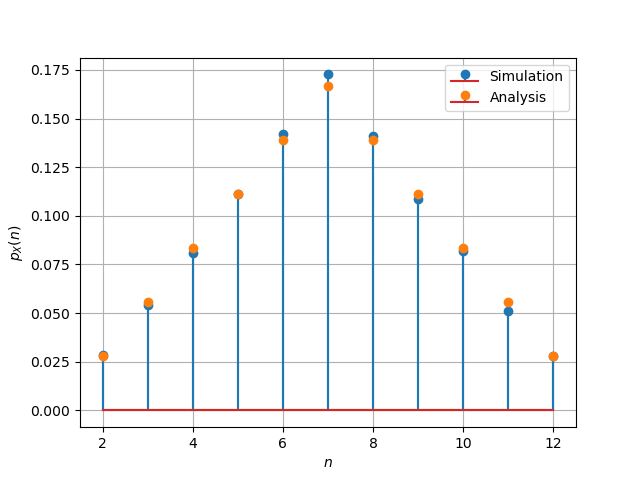
\includegraphics[scale=0.5]{../dig_com/Figs/dice1.png} 
\caption{Plot of $p_X(n)$.  Simulations are close to the analysis. }
\label{fig:dice}
\end{figure}
\item The python code is available in 
\begin{center}
\fbox{\parbox{10.5cm}{\href{https://github.com/AnushaJella/FWC1/blob/main/Digital-communications/codes/chapter3/1_5_dice.py}{/codes/chapter3/1$\_$5$\_$dice.py}}}
\end{center}
\end{enumerate}
\section{Random Variables}
%\numberwithin{equation}{enumi}
\subsection{Uniform Random Numbers}
Let $U$ be a uniform random variable between 0 and 1.
\begin{enumerate}[label=\thesubsection.\arabic*,ref=\thesubsection.\arabic{figure}]%\theenumi]
\item Generate $10^6$ samples of $U$ using a C program and save into a file called uni.dat .
\\
\solution Download the following files and execute the  C program.
\begin{center}
\fbox{\parbox{10.5cm}{\href{https://github.com/AnushaJella/FWC1/blob/main/Digital-communications/codes/chapter4/exrand.c}{/codes/chapter4/exrand.c}}}
\end{center}\begin{center}
\fbox{\parbox{10.5cm}{\href{https://github.com/AnushaJella/FWC1/blob/main/Digital-communications/codes/chapter4/coeffs.h}{/codes/chapter4/coeffs.h}}}
\end{center}
\item
Load the uni.dat file into python and plot the empirical CDF of $U$ using the samples in uni.dat. The CDF is defined as
\begin{align}
F_{U}(x) = \pr{U \le x}
\end{align}
\\
\solution  The following code plot in Fig. \ref{fig:uni_cdf}
\begin{center}
\begin{center}
\fbox{\parbox{10.5cm}{\href{https://github.com/AnushaJella/FWC1/blob/main/Digital-communications/codes/chapter4/uni.dat}{/codes/chapter4/uni.dat}}}
\end{center}
\fbox{\parbox{10.5cm}{\href{https://github.com/AnushaJella/FWC1/blob/main/Digital-communications/codes/chapter4/cdf_plot.py}{/codes/chapter4/cdf$\_$plot.py}}}
\end{center}
\begin{figure}
\centering
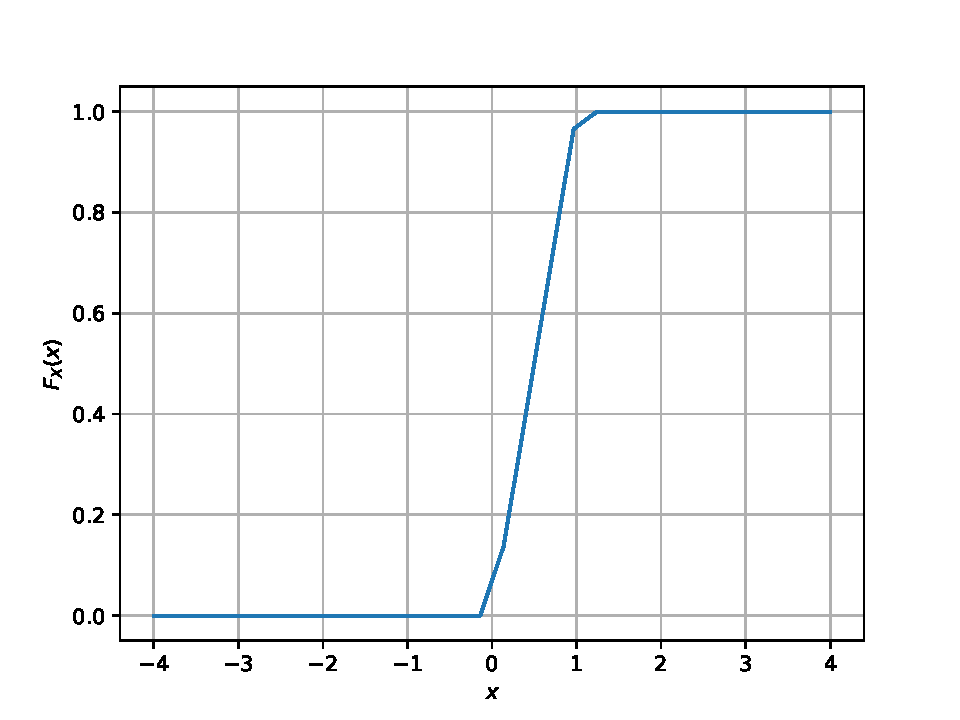
\includegraphics[scale=0.5]{../dig_com/Figs/uni_cdf.pdf} 
\caption{The CDF of $U$}
\label{fig:uni_cdf}
\end{figure}
\item
Find a  theoretical expression for $F_{U}(x)$.
\\
\solution 
\begin{align}
F_{U}(x) &= 
\begin{cases}
0 & x < a \\
\frac{x-a}{b-a} & a \leq x \leq b \\
1 & x \geq b
\end{cases}
\label{eq:dice_x_conv_final}
\end{align}
were, a=0 and b=1.
\item
The mean of $U$ is defined as
%
\begin{equation}
E\sbrak{U} = \frac{1}{N}\sum_{i=1}^{N}U_i
\end{equation}
%
and its variance as
%
\begin{equation}
\text{var}\sbrak{U} = E\sbrak{U- E\sbrak{U}}^2 
\end{equation}
Write a C program to  find the mean and variance of $U$. \\
\solution
\begin{flushleft}
the following C program is used to find mean and variance of uniform distribution .
 \end{flushleft}
 \begin{center}
\fbox{\parbox{10.5cm}{\href{https://github.com/AnushaJella/FWC1/blob/main/Digital-communications/codes/chapter4/uni.dat}{/codes/chapter4/uni.dat}}}
\end{center}
 \begin{center}
\fbox{\parbox{10.5cm}{\href{https://github.com/AnushaJella/FWC1/blob/main/Digital-communications/codes/chapter4/4_1_4_rand.c}{/codes/chapter4/4$\_$1$\_$4$\_$rand.c}}}
\end{center}
\item Verify your result theoretically given that
%
\begin{align}
E\sbrak{U^k} = \int_{-\infty}^{\infty}x^kdF_{U}(x)
\label{eq:expe1}
\end{align}
\solution
\begin{align}
	\label{eq:mean1}
      E\sbrak{X} = \int_{-\infty}^{\infty}xdF_{U}(x) \\
	\label{eq:var1}
	 E\sbrak{X^2} - E^2\sbrak{X} = \int_{-\infty}^{\infty}x^2dF_{U}(x) - \mu^2
\end{align}  
where $\mu$ is the mean and $\sigma$ is variance of random variable.
Substituting the CDF of $U$ from \eqref{eq:dice_x_conv_final} in \eqref{eq:mean1} and \eqref{eq:var1}, we get
\begin{align}
	\label{eq:mean2}
	E\sbrak{X}=\mu &= \frac{1}{2} \\
	\label{eq:var2}
	\sigma_U^2 &= \frac{1}{12}
\end{align} 
\begin{flushleft}
the following python code is used to verify mean and variance of uniform distribution using \eqref{eq:expe1}
 \end{flushleft}
 \begin{flushleft}
 Simulation results:\\
 mean $\mu$ = $\frac{1}{2}$\\
 variance $\sigma^2$= $\frac{1}{12}$
 \end{flushleft}
 \begin{center}
\fbox{\parbox{10.5cm}{\href{https://github.com/AnushaJella/FWC1/blob/main/Digital-communications/codes/chapter4/4_1_5.py}{/codes/chapter4/4$\_$1$\_$5.py}}}
\end{center}
\end{enumerate}
\subsection{Central Limit Theorem}
%
\begin{enumerate}[label=\thesubsection.\arabic*,ref=\thesubsection.\arabic{figure}]
%
\item
Generate $10^6$ samples of the random variable
%
\begin{equation}
X = \sum_{i=1}^{12}U_i -6
\end{equation}
%
using a C program, where $U_i, i = 1,2,\dots, 12$ are  a set of independent uniform random variables between 0 and 1
and save in a file called Gaussian.dat \\
\solution Download the following files and execute the  C program.
\begin{center}
\fbox{\parbox{10.5cm}{\href{https://github.com/AnushaJella/FWC1/blob/main/Digital-communications/codes/chapter4/random_var.c}{/codes/chapter4/random$\_$var.c}}}
\end{center}
\begin{center}
\fbox{\parbox{10.5cm}{\href{https://github.com/AnushaJella/FWC1/blob/main/Digital-communications/codes/chapter4/coeffs.h}{/codes/chapter4/coeffs.h}}}
\end{center}
\item
Load Gaussian.dat in python and plot the empirical CDF of $X$ using the samples in Gaussian.dat. What properties does a CDF have?
\\
\solution The CDF of $X$ is plotted in Fig.\ref{fig:gauss_cdf}
\begin{figure}
\centering
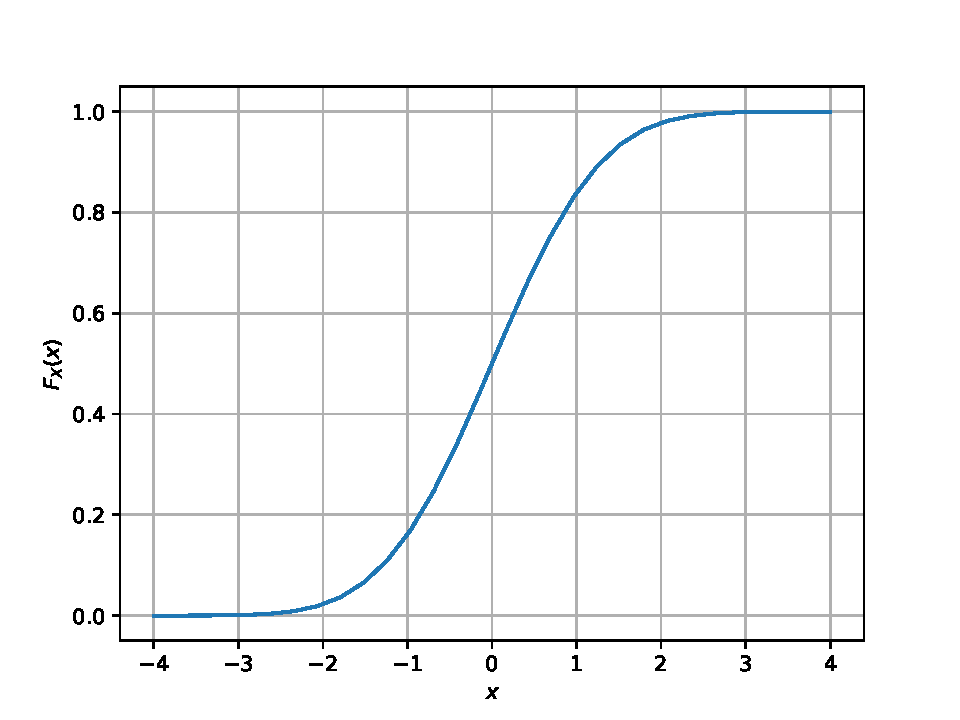
\includegraphics[scale=0.5]{../dig_com/Figs/cdf_clt1.pdf} 
\caption{The CDF of $X$}
\label{fig:gauss_cdf}
\end{figure}
\begin{center}
\fbox{\parbox{10.5cm}{\href{https://github.com/AnushaJella/FWC1/blob/main/Digital-communications/codes/chapter4/cdf_plot_clt.py}{/codes/chapter4/cdf$\_$plot$\_$clt.py}}}
\end{center}
\textbf{Properties:}
\begin{itemize}
\item CDF is non-decreasing function.
\item Maximum value of CDF $F(+\infty)=1$.
\item Minimum value of CDF $F(-\infty)=0$.
\end{itemize}
\item
Load Gaussian.dat in python and plot the empirical PDF of $X$ using the samples in Gaussian.dat. The PDF of $X$ is defined as
\begin{align}
p_{X}(x) = \frac{d}{dx}F_{X}(x)
\end{align}
What properties does the PDF have?
\\
\solution The PDF of $X$ is plotted in Fig. \ref{fig:gauss_pdf} using the code below
\begin{center}
\fbox{\parbox{10.5cm}{\href{https://github.com/AnushaJella/FWC1/blob/main/Digital-communications/codes/chapter4/pdf_plot_clt.py}{/codes/chapter4/pdf$\_$plot$\_$clt.py}}}
\end{center}
\begin{figure}
\centering
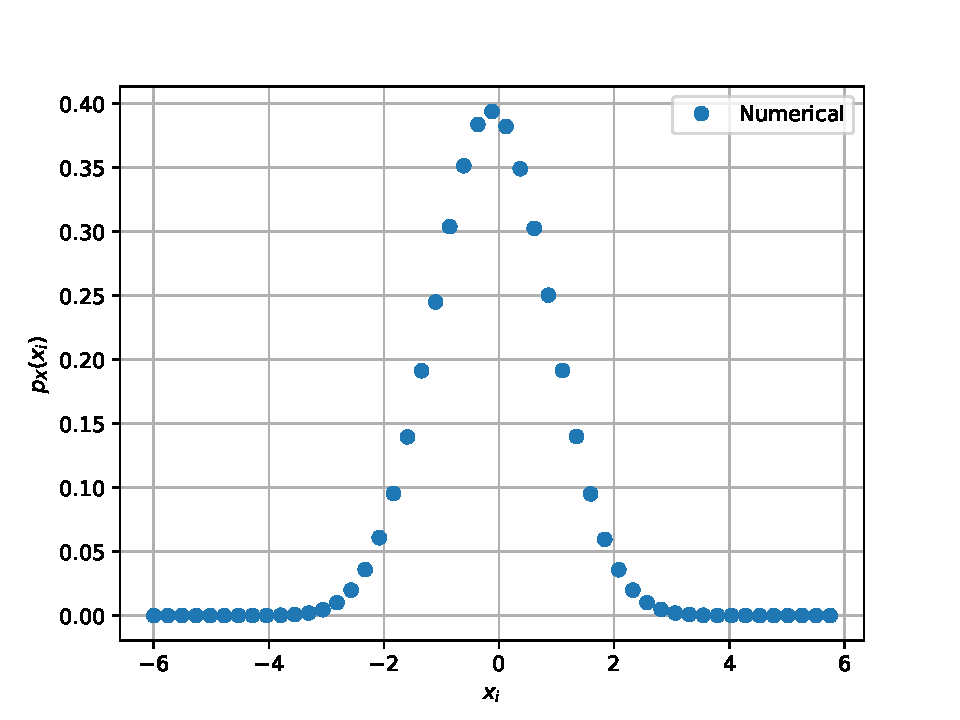
\includegraphics[scale=0.5]{../dig_com/Figs/pdf_clt1.pdf}  
\caption{The PDF of $X$}
\label{fig:gauss_pdf}
\end{figure}
\textbf{Properties} : 
\begin{itemize}
\item Mean,median and mode are equal.
\item The curve is bell-shaped and symmetric about mean.
\item Area under the curve=1.
\end{itemize}
\item Find the mean and variance of $X$ by writing a C program.\\
\solution 
\begin{center}
\fbox{\parbox{10.5cm}{\href{https://github.com/AnushaJella/FWC1/blob/main/Digital-communications/codes/chapter4/random_var.c}{/codes/chapter4/random$\_$var.c}}}
\end{center}
\begin{center}
\fbox{\parbox{10.5cm}{\href{https://github.com/AnushaJella/FWC1/blob/main/Digital-communications/codes/chapter4/coeffs.h}{/codes/chapter4/coeffs.h}}}
\end{center}
\item Given that 
\begin{align}
p_{X}(x) = \frac{1}{\sqrt{2\pi}}\exp\brak{-\frac{x^2}{2}}, -\infty < x < \infty,
\end{align}
repeat the above exercise theoretically.\\
\solution
Mean$(\mu) = E\sbrak{X}$
\begin{align}
    E(X) &= \frac{1}{\sqrt{2\pi}} \int_{-\infty}^{\infty} x e^{-\frac{x^2}{2}}dx\\
    &=0 
\end{align}
\begin{align}
    E\brak{X^2}&= \frac{1}{\sqrt{2\pi}}\int_{-\infty}^{\infty} x^2
e^ {-\frac{x^2}{2}} dx \quad \brak{even function}\\
    &= \frac{2}{\sqrt{2\pi}} \int_{0}^{\infty} x^2 e^{-\frac{x^2}{2}} dx\\
    &= \frac{2}{\sqrt{2\pi}}\int_{0}^{\infty}\sqrt{2u}e^{-u} du \quad\brak{Let \frac{x^2}{2}= u}\\
    &= \frac{2}{\sqrt{\pi}} \int_{0}^{\infty} e^{-u} u^{\frac{3}{2}-1} du\\
    &= \frac{2}{\sqrt{\pi}} \Gamma\brak{{\frac{3}{2}}}\\
    &= \frac{1}{\sqrt{\pi}}\Gamma\brak{\frac{1}{2}} \\
    &= 1
\end{align}
where 
\begin{align}
\Gamma\brak{\frac{1}{2}}=\sqrt{\pi}
\end{align}
%
Thus, the  variance is
\begin{align}
    \sigma^2 =  E\brak X^2 - E^2\brak X = 1
\end{align}
theoretical and numerical plots as shown in fig.\ref{fig:PDF_px}
\begin{center}
\fbox{\parbox{10.5cm}{\href{https://github.com/AnushaJella/FWC1/blob/main/Digital-communications/codes/chapter4/pdf_plot_clt.py}{/codes/chapter4/pdf$\_$plot$\_$clt.py}}}
\end{center}
\begin{figure}
\centering
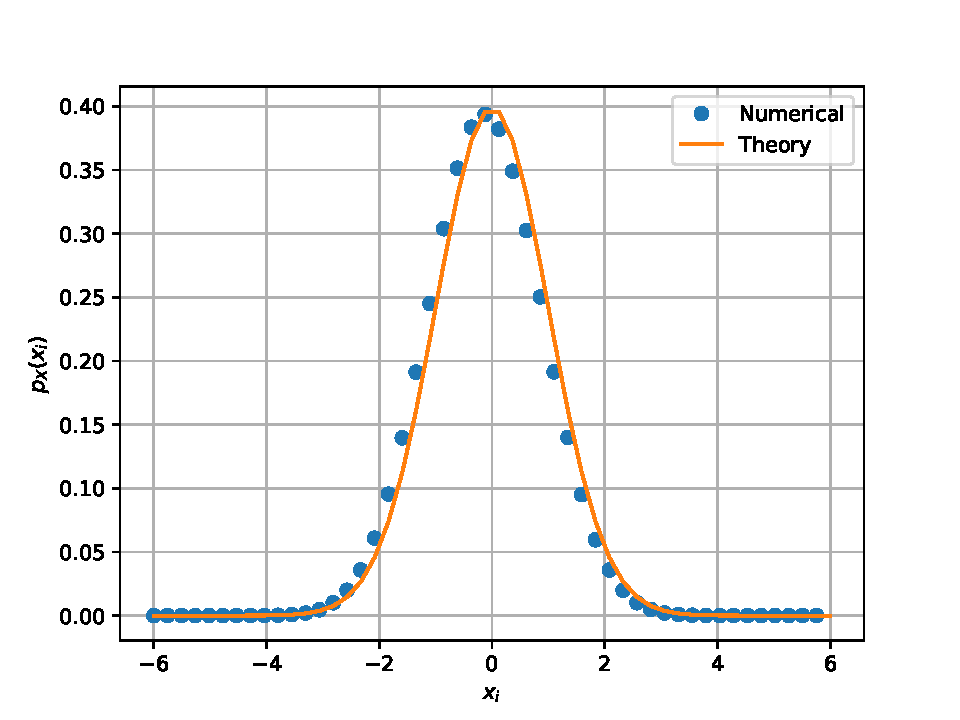
\includegraphics[scale=0.5]{../dig_com/Figs/pdf_clt2.pdf}  
\caption{The PDF of $p\brak{x}$}
\label{fig:PDF_px}
\end{figure}
\end{enumerate}
\subsection{From Uniform to Other}
\begin{enumerate}[label=\thesubsection.\arabic*,ref=\thesubsection.\arabic{figure}]
%
\item
Generate samples of 
%
\begin{equation}
V = -2\ln\brak{1-U}
\end{equation}
%
and plot its CDF. \\
\solution 
The CDF plot of V is in fig.\ref{fig:CDF_uni_V}
\begin{center}
\fbox{\parbox{10.5cm}{\href{https://github.com/AnushaJella/FWC1/blob/main/Digital-communications/codes/chapter4/uniform_numbers.c}{/codes/chapter4/uniform$\_$var.c}}}
\end{center}
\begin{center}
\fbox{\parbox{10.5cm}{\href{https://github.com/AnushaJella/FWC1/blob/main/Digital-communications/codes/chapter4/coeffs.h}{/codes/chapter4/coeffs.h}}}
\end{center}
\begin{center}
\fbox{\parbox{10.5cm}{\href{https://github.com/AnushaJella/FWC1/blob/main/Digital-communications/codes/chapter4/uni.dat}{/codes/chapter4/uni.dat}}}
\end{center}
\begin{center}
\fbox{\parbox{10.5cm}{\href{https://github.com/AnushaJella/FWC1/blob/main/Digital-communications/codes/chapter4/cdf_plot_uni.py}{/codes/chapter4/cdf$\_$plot$\_$uni.py}}}
\end{center}
\begin{figure}
\centering
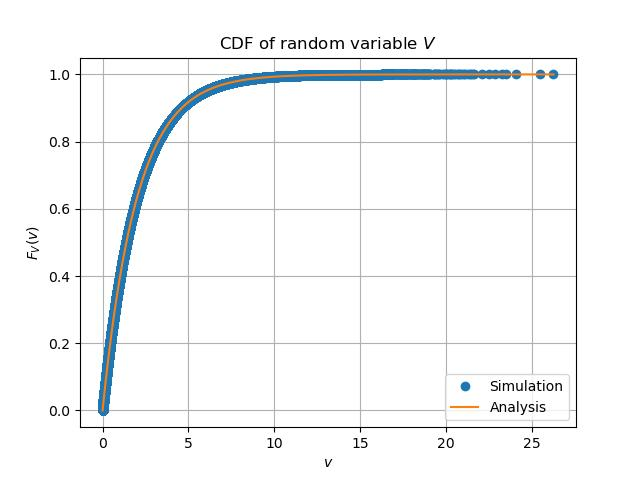
\includegraphics[scale=0.5]{../dig_com/Figs/cdf_uni_othr.jpg}  
\caption{The CDF of $V$}
\label{fig:CDF_uni_V}
\end{figure}
\item Find a theoretical expression for $F_V(x)$.\\
\solution
\begin{align*}
F_{V}(x) = \pr{V \le x}\\
 =\pr{-2\ln\brak{1-U} \le x}\\
 =\pr{(1-U)\le e^{\frac{-x}{2}}}\\
 F_U(x)=\pr{U \le 1-e^{\frac{-x}{2}}}
\end{align*}
\begin{center}
\fbox{\parbox{10.5cm}{\href{https://github.com/AnushaJella/FWC1/blob/main/Digital-communications/codes/chapter4/cdf_plot_uni.py}{/codes/chapter4/cdf$\_$plot$\_$uni.py}}}
\end{center}
\end{enumerate}
\subsection{Triangular Distribution}
\begin{enumerate}[label=\thesubsection.\arabic*,ref=\thesubsection.\arabic{figure}]
%
\item Generate 
	\begin{align}
		T = U_1+U_2
	\end{align}
\solution
\begin{center}
\fbox{\parbox{10.5cm}{\href{https://github.com/AnushaJella/FWC1/blob/main/Digital-communications/codes/chapter4/tri.c}{/codes/chapter4/tri.c}}}
\end{center}
\begin{center}
\fbox{\parbox{10.5cm}{\href{https://github.com/AnushaJella/FWC1/blob/main/Digital-communications/codes/chapter4/coeffs.h}{/codes/chapter4/coeffs.h}}}
\end{center}
\begin{center}
\fbox{\parbox{10.5cm}{\href{https://github.com/AnushaJella/FWC1/blob/main/Digital-communications/codes/chapter4/Uni1.dat}{/codes/chapter4/uni1.dat}}}
\end{center}
\begin{center}
\fbox{\parbox{10.5cm}{\href{https://github.com/AnushaJella/FWC1/blob/main/Digital-communications/codes/chapter4/Uni2.dat}{/codes/chapter4/uni2.dat}}}
\end{center}
\item Find the CDF of $T$.\\
\solution
For following CDF python code plot is as shown in Fig.\ref{fig:tri_cdf11}\\ 
\begin{center}
\fbox{\parbox{10.5cm}{\href{https://github.com/AnushaJella/FWC1/blob/main/Digital-communications/codes/chapter4/T.dat}{/codes/chapter4/T.dat}}}
\end{center}
\begin{center}
\fbox{\parbox{10.5cm}{\href{https://github.com/AnushaJella/FWC1/blob/main/Digital-communications/codes/chapter4/cdf_plot_tri.py}{/codes/chapter4/cdf$\_$plot$\_$tri.py}}}
\end{center}
\begin{figure}
\centering
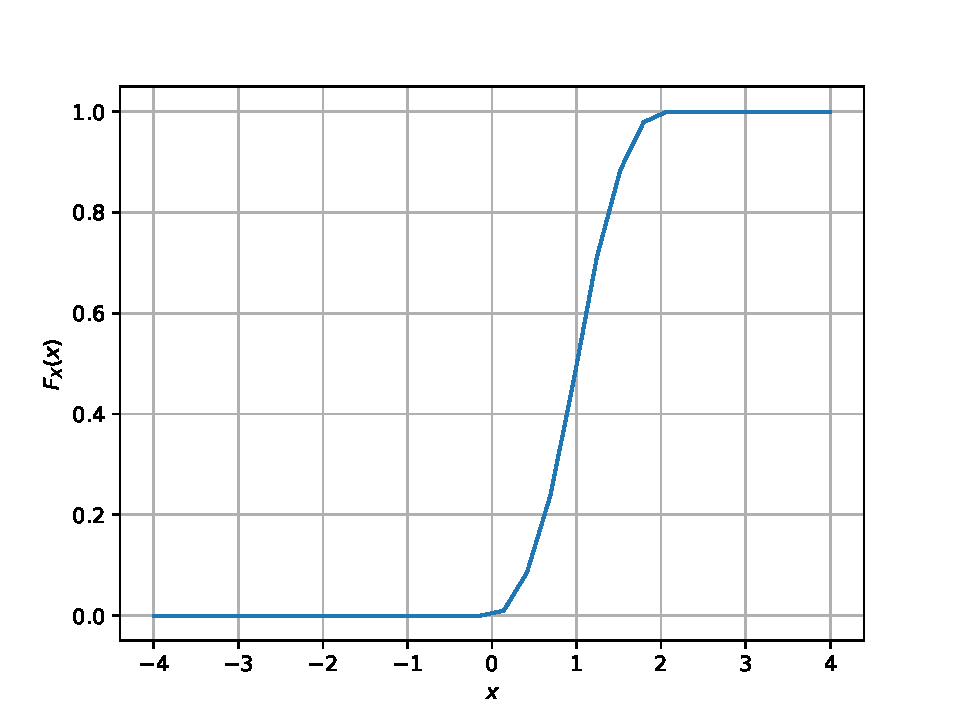
\includegraphics[scale=0.5]{../dig_com/Figs/tri_cdf1.pdf} 
\caption{The CDF of $T$}
\label{fig:tri_cdf11}
\end{figure}
\item Find the PDF of $T$.\\
\solution: The following PDF python code is to plot Fig.\ref{fig:tri_pdf11}
\begin{center}
\fbox{\parbox{10.5cm}{\href{https://github.com/AnushaJella/FWC1/blob/main/Digital-communications/codes/chapter4/T.dat}{/codes/chapter4/T.dat}}}
\end{center}
\begin{center}
\fbox{\parbox{10.5cm}{\href{https://github.com/AnushaJella/FWC1/blob/main/Digital-communications/codes/chapter4/cdf_plot_tri.py}{/codes/chapter4/pdf$\_$plot$\_$tri.py}}}
\end{center}
\begin{figure}
\centering
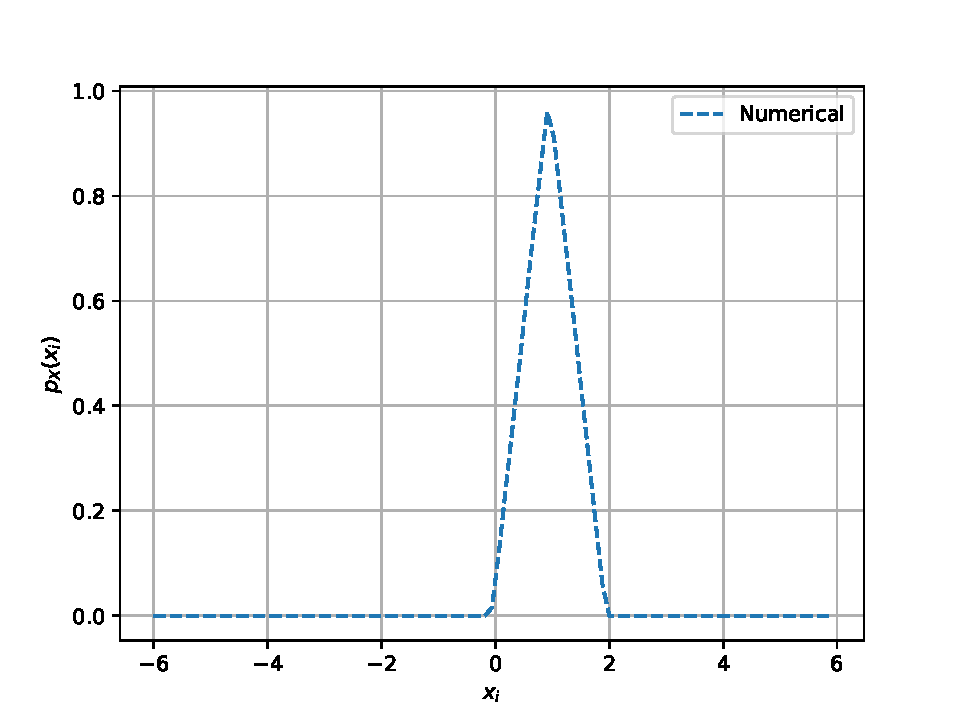
\includegraphics[scale=0.5]{../dig_com/Figs/tri_pdf1.pdf} 
\caption{The CDF of $T$}
\label{fig:tri_pdf11}
\end{figure}
\item Find the theoretical expressions for the PDF and CDF of $T$.\\
\solution
CDF $F_U(x)$ is
\begin{align}
F_{T}(x) &= 
\begin{cases}
0 & x \leq a \\
\frac{(x-a)^2}{(b-a)(c-a)} & a < x \leq c \\
1-\frac{(b-x)^2}{(b-a)(c-a)} & c < x \leq b\\
1 & x > b
\end{cases}
\end{align}
PDF $p_T(x)$
\begin{align}
p_{T}(x) = \frac{d}{dx}F_{T}(x)
\end{align}
\begin{align}
p_{T}(x) &= 
\begin{cases}
0 & x \leq a \\
\frac{2(x-a)}{(b-a)(c-a)} & a < x \leq c \\
\frac{2(b-x)}{(b-a)(c-a)} & c < x \leq b\\
0 & x > b
\end{cases}
\end{align}
\item Verify your results through a plot. \\
\solution 
Compare theoretical and simulation results of CDF and PDF of triangular distribution using following python codes as given below and plots as shown in \ref{fig:tri_cdf},\ref{fig:triangular_pdf}.
\begin{center}
\fbox{\parbox{10.5cm}{\href{https://github.com/AnushaJella/FWC1/blob/main/Digital-communications/codes/chapter4/cdf_plot_tri2.py}{/codes/chapter4/cdf$\_$plot$\_$tri2.py}}}
\end{center}
\begin{center}
\fbox{\parbox{10.5cm}{\href{https://github.com/AnushaJella/FWC1/blob/main/Digital-communications/codes/chapter4/pdf_plot_tri2.py}{/codes/chapter4/pdf$\_$plot$\_$tri2.py}}}
\end{center}
\begin{figure}
\centering
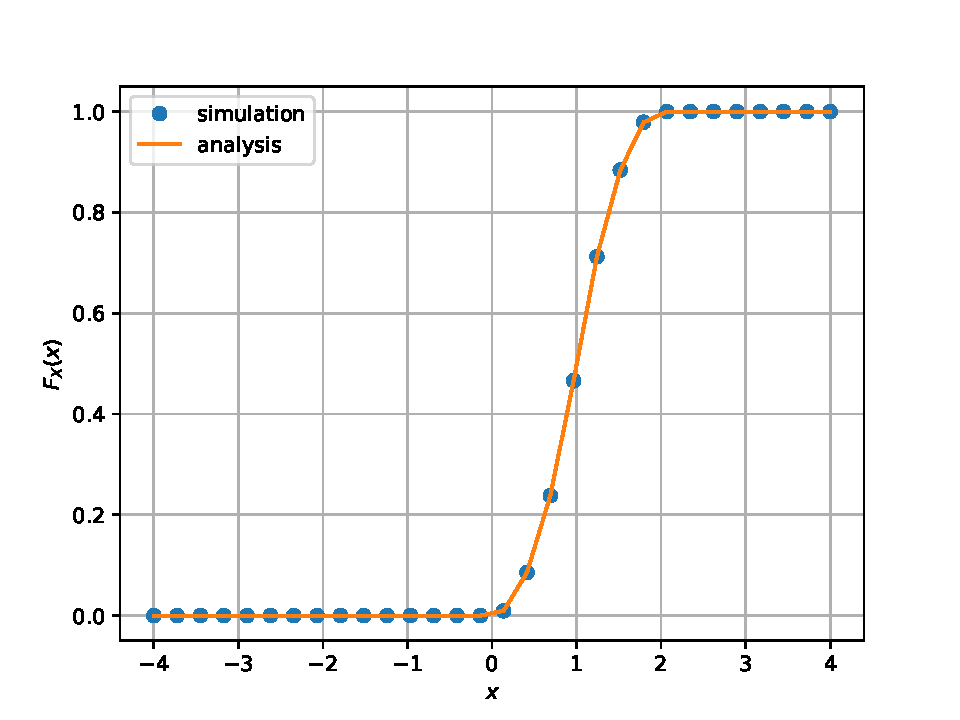
\includegraphics[scale=0.5]{../dig_com/Figs/tri_cdf2.pdf} 
\caption{The CDF of $T$}
\label{fig:tri_cdf}
\end{figure}
\begin{figure}
\centering
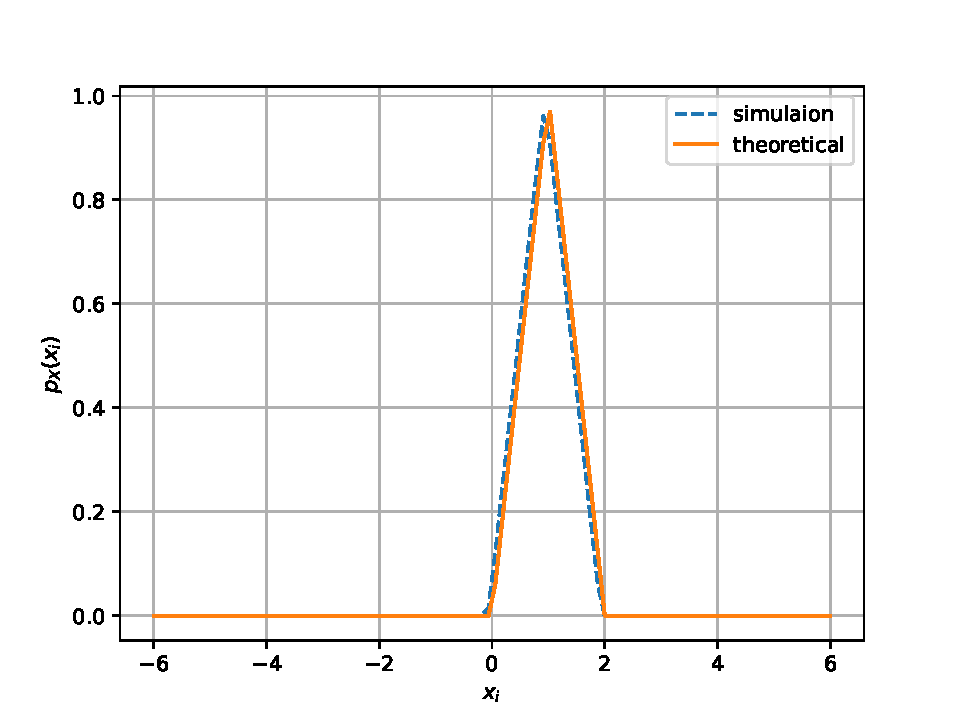
\includegraphics[scale=0.5]{../dig_com/Figs/tri_pdf2.pdf} 
\caption{The PDF of $T$}
\label{fig:triangular_pdf}
\end{figure}
\end{enumerate}
%%% chapter-3%%%
\section{Maximum Likelyhood Detection:BPSK}
\subsection{Maximum Likelihood}
\begin{enumerate}[label=\thesubsection.\arabic*,ref=\thesubsection.\arabic{figure}]
\item Generate equiprobable $X \in \cbrak{1,-1}$.\\
\solution
\begin{center}
\fbox{\parbox{10.5cm}{\href{https://github.com/AnushaJella/FWC1/blob/main/Digital-communications/codes/chapter5/5_1_1.py}{/codes/chapter4/5$\_$1$\_$1.py}}}
\end{center}
%
\item Generate 
\begin{equation}
Y = AX+N,
\end{equation}
		where $A = 5$ dB,  and $N \sim \gauss{0}{1}$.
\begin{center}
\fbox{\parbox{10.5cm}{\href{https://github.com/AnushaJella/FWC1/blob/main/Digital-communications/codes/chapter5/5_1_2.py}{/codes/chapter5/5$\_$1$\_$2.py}}}
\end{center}		
\item Plot $Y$ using a scatter plot.\\
\solution
Code for plot of $Y$ using scatter plot is given below and it's plot is in fig.\ref{fig:scatter1} 
\begin{figure}
\centering
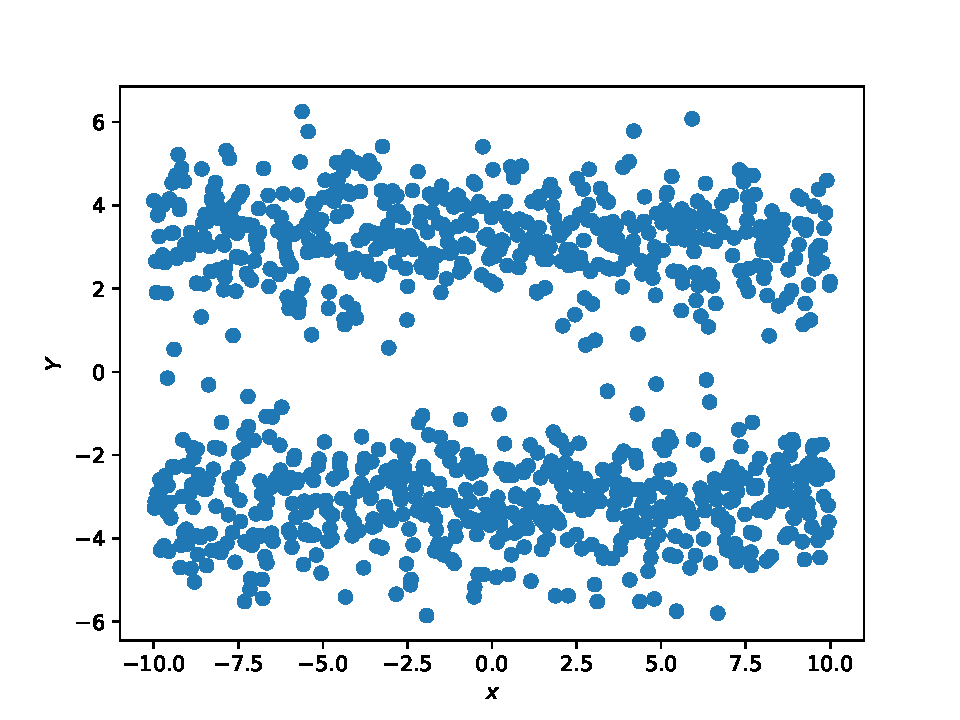
\includegraphics[scale=0.5]{../dig_com/Figs/Y_scatter5.pdf}  
\caption{The scatter plot of Y}
\label{fig:scatter1}
\end{figure}
\begin{center}
\fbox{\parbox{10.5cm}{\href{https://github.com/AnushaJella/FWC1/blob/main/Digital-communications/codes/chapter5/5_1_3.py}{/codes/chapter5/5$\_$1$\_$3.py}}}
\end{center}
	\item Guess how to estimate $X$ from $Y$.\\
	\solution 
	Given two signals are represented by two signals\\
	'1' for X=1 and\\
	'0' for X=-1.
	according to decision rule $P(Y > y)$
	\begin{align}
        y \dec{1}{-1} 0 \label{eq:decision1}
        \end{align}
\item
\label{ml-ch4_sim}
Find 
\begin{equation}
	P_{e|0} = \pr{\hat{X} = -1|X=1}
\end{equation}
and 
\begin{equation}
	P_{e|1} = \pr{\hat{X} = 1|X=-1}
\end{equation}\\
\solution From above problem solution \eqref{eq:decision1}\\
\begin{align*}
P_{e|0} = \pr{\hat{X} = -1|X=1}\\
   = \pr{Y<0|X=1}\\
   = \pr{AX+N<0|X=1}\\
   = \pr{A+N<0}\\
    =\pr{N<-A}   
\end{align*}
\begin{align*}
P_{e|1} = \pr{\hat{X} = 1|X=-1}\\
   = \pr{Y>0|X=-1}\\
   = \pr{AX+N>0|X=-1}\\
   = \pr{-A+N>0}\\
    =\pr{N>A}   
\end{align*}
where,$N \sim \gauss{0}{1}$\\
\begin{align}
 \therefore \pr{N>A}=\pr{N<-A}\\
 P_{e|0}=P_{e|1} \label{eq:equi_prob}
\end{align}
 \item Find $P_e$ assuming that $X$ has equiprobable symbols.\\
 \solution \begin{align}
	P_e &= \pr{X=1}P_{e|1} + \pr{X=-1}P_{e|0}& \label{eq:Pe_of_X}
	\end{align}
	\text{given $X$ is equiprobable}\\
	\begin{align}
	P_e &= \frac{1}{2}P_{e|1} + \frac{1}{2}P_{e|0}
\end{align}
Substituting from \eqref{eq:equi_prob}
\begin{equation}
	P_e = \pr{N > A}
\end{equation}
Given a random varible $X \sim \gauss{0}{1}$ the Q-function is defined as
\begin{align}
	Q(x) &= \pr{X > x}\\
	\label{eq:q_func_integral}
	Q(x) &= \frac{1}{\sqrt{2\pi}} \int_x^\infty \exp\left(-\frac{u^2}{2}\right) \, du.
\end{align}
Using the Q-function, $P_e$ is rewritten as
\begin{equation}
	P_e = Q(A)
\end{equation} 
\item
Verify by plotting  the theoretical $P_e$ with respect to $A$ from 0 to 10 dB.\\
\solution 
theoretical and simulation results are shown in \ref{fig:bpsk1}
\begin{center}
\fbox{\parbox{10.5cm}{\href{https://github.com/AnushaJella/FWC1/blob/main/Digital-communications/codes/chapter5/5_1_7.py}{/codes/chapter5/5$\_$1$\_$7.py}}}
\end{center}
\begin{figure}
\centering
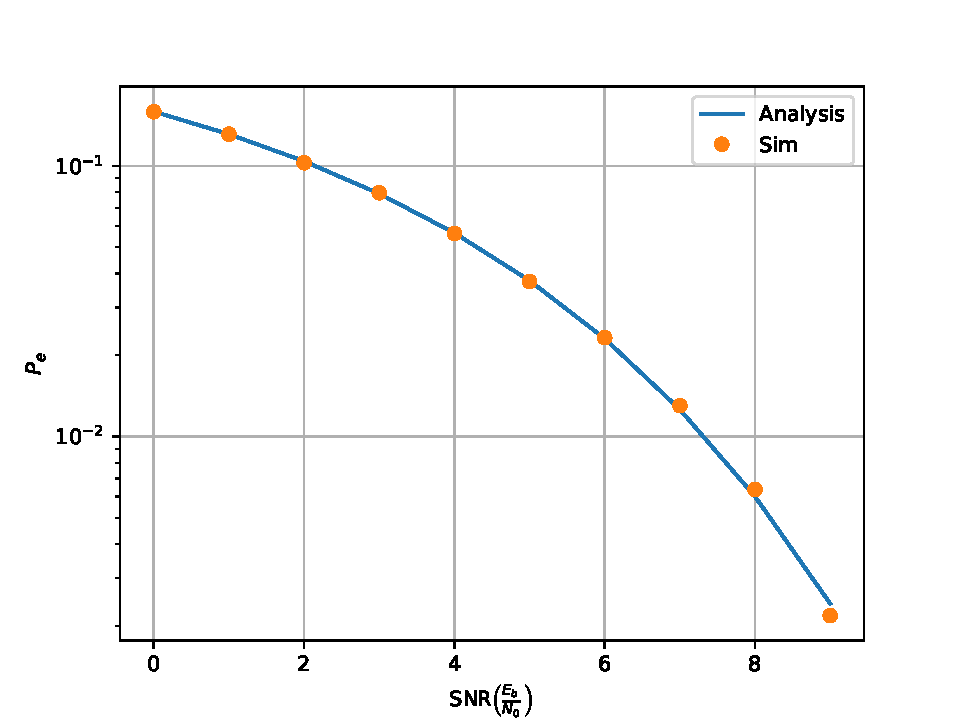
\includegraphics[scale=0.5]{../dig_com/Figs/bpsk_ber.pdf}   
\caption{$P_e$ of X wrt SNR(A)}
\label{fig:bpsk1}
\end{figure}
\item Now, consider a threshold $\delta$  while estimating $X$ from $Y$. Find the value of $\delta$ that maximizes the theoretical $P_e$.\\
\solution From \ref{eq:decision1} the decision rule, 
\begin{equation}
y \dec{1}{-1} \delta
\end{equation}
\begin{align*}
	P_{e|0} &= \pr{\hat{X} = -1|X=1}&\\
	&= \pr{Y < \delta|X=1}&\\
	&= \pr{AX + N < \delta|X=1}&\\ 
	&= \pr{A + N < \delta}&\\
	&= \pr{N < -A + \delta}&\\
	&= \pr{N > A - \delta}&\\
	&= Q(A-\delta)
\end{align*}
\begin{align*}
	P_{e|1} &= \pr{\hat{X} = 1|X=-1}&\\
	&= \pr{Y > \delta|X=-1}&\\
	&= \pr{N > A + \delta}&\\
	&= Q(A+\delta)
\end{align*}
Using \ref{eq:Pe_of_X} $P_e$ is given by
\begin{align}
	P_e &= \frac{1}{2}Q(A+\delta) + \frac{1}{2}Q(A-\delta)
\end{align}
Using the integral for Q-function from \ref{eq:q_func_integral},
\begin{align}
	P_e &= k(\int_{A+\delta}^\infty \exp\left(-\frac{u^2}{2}\right) \, du + \int_{A-\delta}^\infty \exp\left(-\frac{u^2}{2}\right) \, du)
	\label{eq:Pe_in_q}
	\end{align}
	\text{where k is a constant}	\\
Differentiating \ref{eq:Pe_in_q}. wrt $\delta$ (using Leibniz's rule) and equating to $0$, we get
\begin{align*}
	\exp\left(-\frac{(A+\delta)^2}{2}\right)-\exp\left(-\frac{(A-\delta)^2}{2}\right) &= 0&\\
	\frac{\exp\left(-\frac{(A+\delta)^2}{2}\right)}{\exp\left(-\frac{(A-\delta)^2}{2}\right)} &= 1&\\
	\exp\left(-\frac{(A+\delta)^2-(A-\delta)^2}{2}\right) &= 1&\\
	\exp\left(-2A\delta\right) &= 1&\\
	\intertext{Taking $\log$ on both sides}\\
	-2A\delta &= 0&\\
	\implies \delta &= 0
\end{align*}
$P_e$ is maximum for $\delta = 0$
\item Repeat the above exercise when 
	\begin{align}
		p_{X}(0) = p
	\end{align}
	\solution Given $X$ is not equiprobable, $P_e$ is given by,
\begin{align}
	P_e &= (1-p)P_{e|1} + pP_{e|0}&\\
	&= (1-p)Q(A+\delta) + pQ(A-\delta)
\end{align}
Using the integral for Q-function from \ref{eq:q_func_integral}
\begin{align}
	P_e = k((1-p)\int_{A+\delta}^\infty \exp\left(-\frac{u^2}{2}\right) \, du + 
	p\int_{A-\delta}^\infty \exp\left(-\frac{u^2}{2}\right) \, du)
\end{align}
where $k$ is a constant.\\
differentiate $P_e$ wrt $\delta$ and equate to zero,
\begin{align*}
	(1-p)\exp\left(-\frac{(A+\delta)^2}{2}\right)-p\exp\left(-\frac{(A-\delta)^2}{2}\right) &= 0&\\
	\frac{\exp\left(-\frac{(A+\delta)^2}{2}\right)}{\exp\left(-\frac{(A-\delta)^2}{2}\right)} &= \frac{p}{(1-p)}&\\
	\exp\left(-\frac{(A+\delta)^2-(A-\delta)^2}{2}\right) &= \frac{p}{(1-p)}&\\
	\exp\left(-2A\delta\right) &= \frac{p}{(1-p)}&\\
	\intertext{Taking $\log$ on both sides}\\
	\delta = \frac{1}{2A}\log\left(\frac{1}{p}-1\right)
\end{align*}
\end{enumerate}
%
%%%chapter-4%%
\section{Transformation of random variables}	
\subsection{Gaussian to Other}
\begin{enumerate}[label=\thesubsection.\arabic*,ref=\thesubsection.\arabic{figure}]
\item
Let $X_1 \sim  \gauss{0}{1}$ and $X_2 \sim  \gauss{0}{1}$. Plot the CDF and PDF of
%
\begin{equation}
V = X_1^2 + X_2^2
\end{equation}
\solution 
The plots of CDF and PDF of V as shown in fig.\ref{fig:gauss_cdf1} , \ref{fig:gauss_pdf1} respectively.
\begin{center}
\fbox{\parbox{10.5cm}{\href{https://github.com/AnushaJella/FWC1/blob/main/Digital-communications/codes/chapter6/6_1_cdf.py}{/codes/chapter6/6$\_$1$\_$cdf.py}}}
\end{center}
\begin{center}
\fbox{\parbox{10.5cm}{\href{https://github.com/AnushaJella/FWC1/blob/main/Digital-communications/codes/chapter6/6_1_pdf.py}{/codes/chapter6/6$\_$1$\_$pdf.py}}}
\end{center}
\begin{figure}
\centering
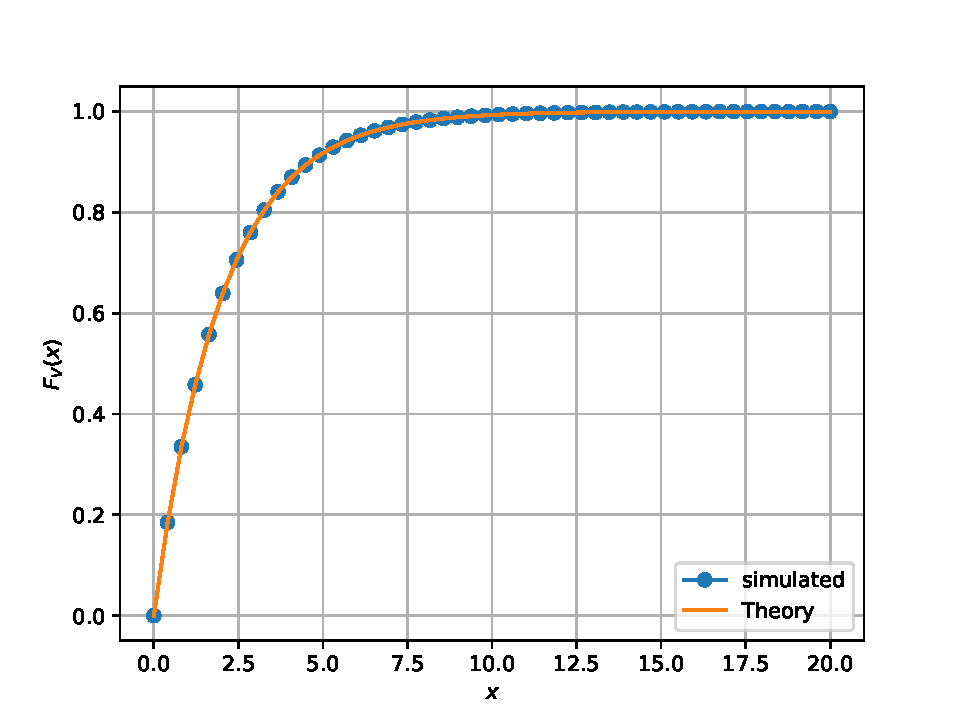
\includegraphics[scale=0.5]{../dig_com/Figs/gau_othr_cdf.pdf}  
\caption{The CDF of $V$}
\label{fig:gauss_cdf1}
\end{figure}
\begin{figure}
\centering
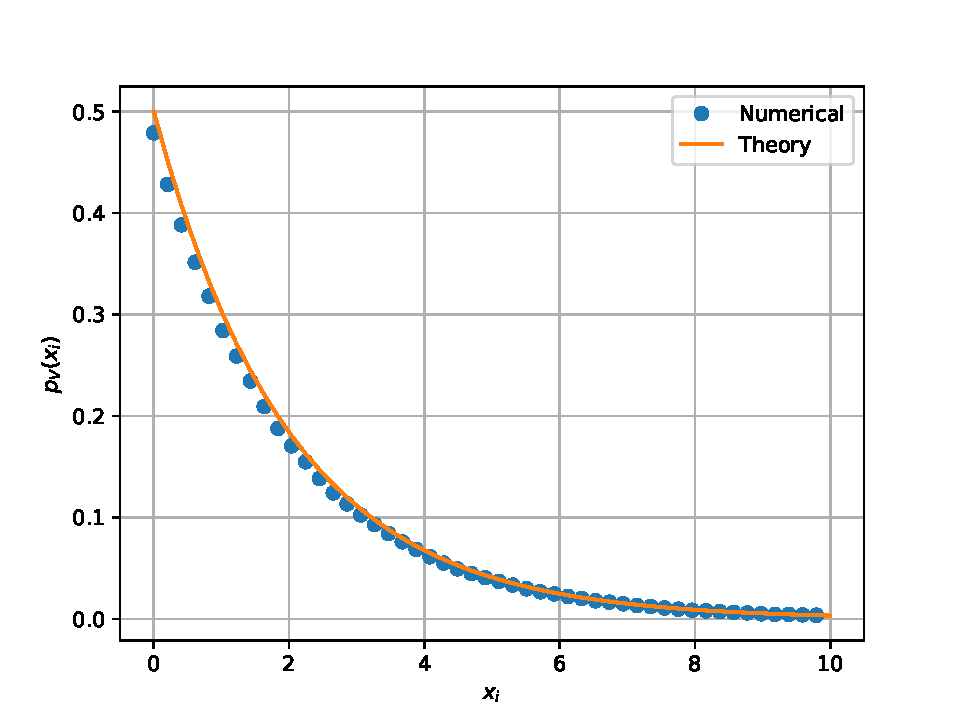
\includegraphics[scale=0.5]{../dig_com/Figs/gau_othr_pdf.pdf}   
\caption{The PDF of $V$}
\label{fig:gauss_pdf1}
\end{figure}
\item
If
%
\begin{equation}
F_{V}(x) = 
\begin{cases}
1 - e^{-\alpha x} & x \geq 0 \\
0 & x < 0,
\end{cases}
\end{equation}
%
find $\alpha$.\\
\solution
\begin{center}
\fbox{\parbox{10.5cm}{\href{https://github.com/AnushaJella/FWC1/blob/main/Digital-communications/codes/chapter6/6_2_cdf.py}{/codes/chapter6/6$\_$2$\_$cdf.py}}}
\end{center}
\begin{figure}
\centering
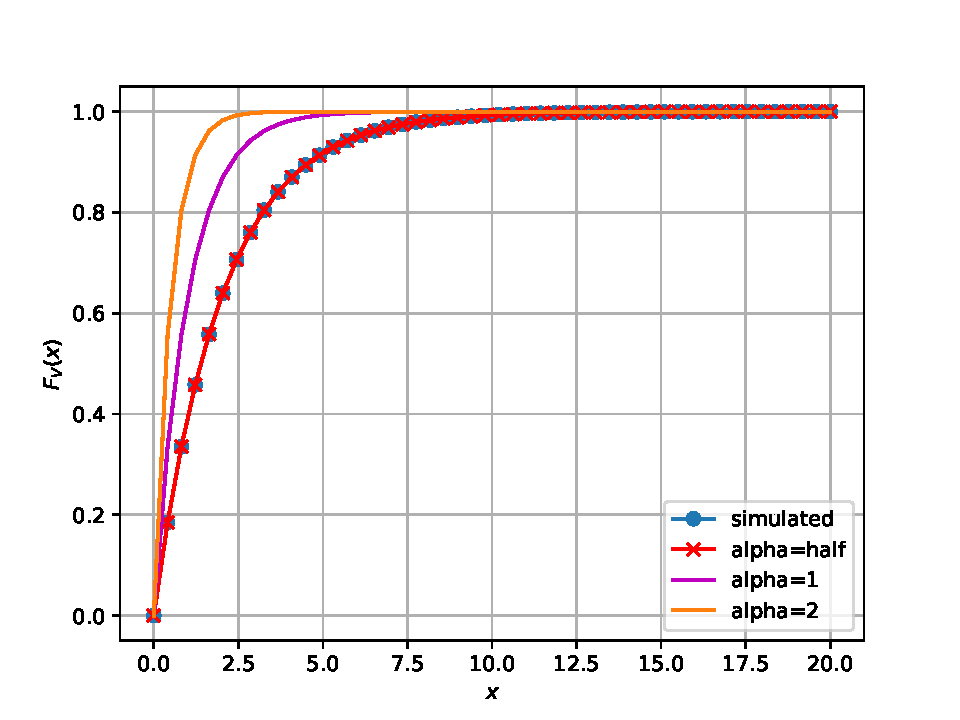
\includegraphics[scale=0.5]{../dig_com/Figs/gau_othr_alpha.pdf}    
\caption{The CDF of $V$ for different alpha}
\label{fig:gauss_cdf_alpha}
\end{figure}
from \ref{fig:gauss_cdf_alpha}
$alpha$= 0.5
\item
\label{ch3_raleigh_sim}
Plot the CDF and PDf of
%
\begin{equation}
A = \sqrt{V}
\end{equation}\\
\solution
CDF,PDF plots are as shown in \ref{fig:gauss_othr_cdf2},\ref{fig:gauss_othr_pdf2}
\begin{center}
\fbox{\parbox{10.5cm}{\href{https://github.com/AnushaJella/FWC1/blob/main/Digital-communications/codes/chapter6/6_3_cdf.py}{/codes/chapter6/6$\_$3$\_$cdf.py}}}
\end{center}
\begin{center}
\fbox{\parbox{10.5cm}{\href{https://github.com/AnushaJella/FWC1/blob/main/Digital-communications/codes/chapter6/6_3_pdf.py}{/codes/chapter6/6$\_$3$\_$pdf.py}}}
\end{center}
\begin{figure}
\centering
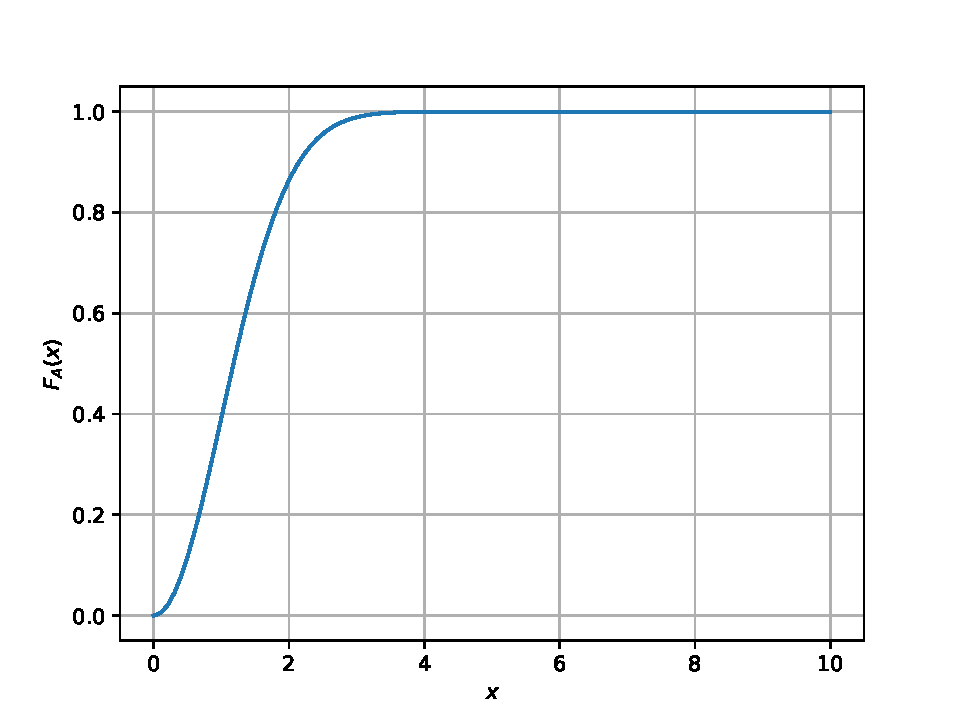
\includegraphics[scale=0.5]{../dig_com/Figs/gau_othr_cdf2.pdf}     
\caption{The CDF of $A$ }
\label{fig:gauss_othr_cdf2}
\end{figure}
\begin{figure}
\centering
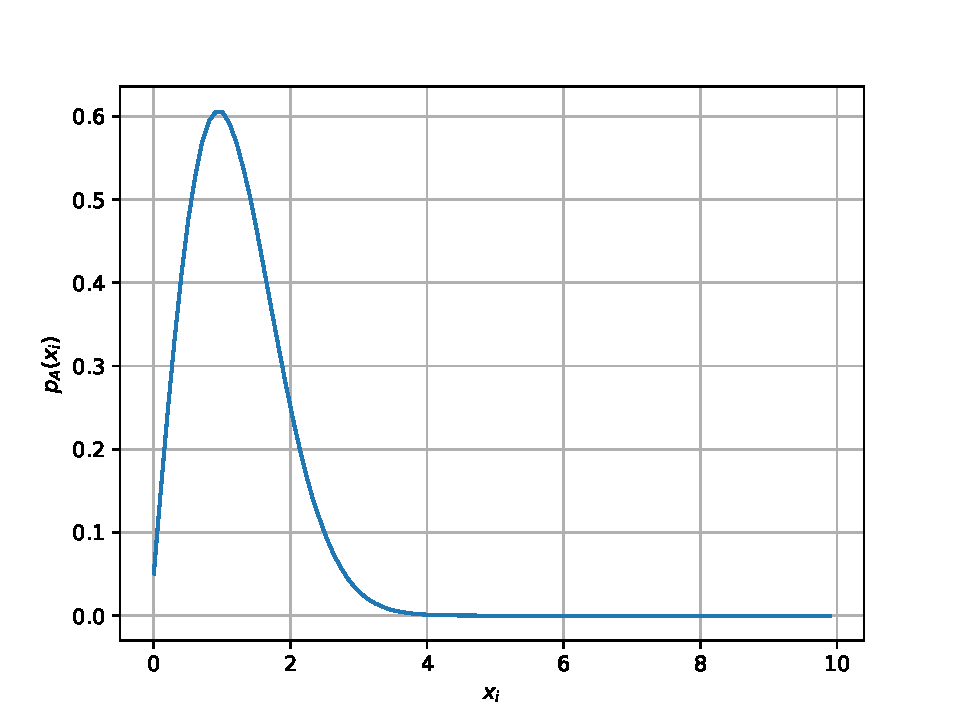
\includegraphics[scale=0.5]{../dig_com/Figs/gau_othr_pdf2.pdf}     
\caption{The PDF of $A$ }
\label{fig:gauss_othr_pdf2}
\end{figure}
\end{enumerate}

\subsection{Conditional Probability}
\begin{enumerate}[label=\thesubsection.\arabic*,ref=\thesubsection.\arabic{figure}]
\item
\label{ch4_sim}
Plot 
\begin{equation}
P_e = \pr{\hat{X} = -1|X=1}
\end{equation}
%
for 
\begin{equation}
Y = AX+N,
\end{equation}
where $A$ is Raleigh with $E\sbrak{A^2} = \gamma, N \sim \gauss{0}{1}, X \in \brak{-1,1}$ for $0 \le \gamma \le 10$ dB.
\item
Assuming that $N$ is a constant, find an expression for $P_e$.  Call this $P_e(N)$\\
\solution The estimated value $\hat{X}$ is given by
\begin{align}
\hat{X} = 
\begin{cases}
+1 & Y>0\\
-1 & Y<0
\end{cases}
\end{align}
For $X = 1$, 
\begin{align}
Y &= A + N\\
P_e &= \pr{\hat{X} = -1|X=1} \\
&= \pr{Y<0 |X=1}\\
&= \pr{A<-N}\\
&= F_A(-N)\\
&= \int_{-\infty}^{-N} f_A(x)dx
\end{align}
By definition
\begin{align}
f_A(x) = 
\begin{cases}
\frac{x}{\sigma^2}\exp\brak{{-\frac{x^2}{2\sigma^2}}} & x\geq0\\
0 & otherwise
\end{cases}
\end{align}
If $N>0, f_A(x) = 0$. Then,
\begin{align}
 P_e=0  
\end{align}
If $N<0$. Then,
\begin{align}
 P_e(N) &=\int_{-\infty}^{-N} f_A(x)dx\\
 &=\int_{-\infty}^{0} 0dx+\int_{0}^{-N} f_A(x)dx\\
 &=\int_{0}^{-N} \frac{x}{\sigma^2}\exp\brak{{-\frac{x^2}{2\sigma^2}}}dx\\
 &=1-\exp{\brak{-\frac{N^2}{2\sigma^2}}}
\end{align}
Therefore,
\begin{align}\label{pe(N)}
P_e(N) = 
\begin{cases}
1-\exp\brak{{-\frac{N^2}{2\sigma^2}}} & N<0\\
0 & otherwise
\end{cases}
\end{align}
%
\item
%
\label{ch4_anal}
For a function $g$,
\begin{equation}
E\sbrak{g(X)} = \int_{-\infty}^{\infty}g(x)p_{X}(x)\, dx
\end{equation}
%
Find $P_e = E\sbrak{P_e(N)}$.
\\
\solution
Since $N \sim \gauss{0}{1}$ ,
\begin{align}
  p_N(x)= \frac{1}{\sqrt{2\pi}}\exp \brak{-\frac{x^2}{2} }
\end{align}
And from \eqref{pe(N)} 
\begin{align}
    P_e(x)=
    \begin{cases}
1-\exp\brak{{-\frac{x^2}{2\sigma^2}}} & x<0\\
0 & otherwise
\end{cases}
\end{align}

\begin{align}
 P_e=E\sbrak{P_e(N)} = \int_{-\infty}^{\infty}P_e(x)p_{N}(x)\, dx  
\end{align}
If $x<0, P_e(x)=0$ and using the fact that for an even function
\begin{align}
\int_{-\infty}^{\infty}f(x)=2\int_{-\infty}^{0}f(x)   
\end{align}
we get
\begin{align}
  P_e&= \frac{1}{\sqrt{2\pi}}\int_{-\infty}^{0}\exp \brak{ -\frac{x^2}{2}} \brak{1-\exp \brak{ -\frac{x^2}{2\sigma^2}} } dx\\
&= \frac{1}{2\sqrt{2\pi}} \int_{-\infty}^{\infty} \exp \brak{ -\frac{x^2}{2} }dx \nonumber \\
&- \frac{1}{2\sqrt{2\pi}} \int_{-\infty}^{\infty} \exp \brak{-\frac{(1+ \sigma^2)x^2}{2 \sigma^2}}  dx\\
&= \frac{\sqrt{2\pi} - \sqrt{\frac{\pi(2\sigma^2)}{1+\sigma^2}}}{2\sqrt{2\pi}}\\
&= \frac{1}{2} - \frac{1}{2}\sqrt{\frac{\sigma^2}{1+\sigma^2}}
\end{align}
For a Rayleigh Distribution with scale $= \sigma$,
\begin{align}
E\sbrak{A^2} = 2\sigma^2\\
\gamma = 2\sigma^2\\
\therefore P_e = \frac{1}{2} - \frac{1}{2}\sqrt{\frac{\gamma}{2+\gamma}}
\end{align}
\item
Plot $P_e$ in problems \ref{ch4_sim} and \ref{ch4_anal} on the same graph w.r.t $\gamma$.  Comment. \\
\solution $P_e$ is plotted w.r.t $\gamma$ in \ref{fig:Pe_gamma1} using the code below.
\begin{center}
\fbox{\parbox{10.5cm}{\href{https://github.com/AnushaJella/FWC1/blob/main/Digital-communications/codes/chapter6/6_2_4_pe.py}{/codes/chapter6/6$\_$2$\_$4$\_$pe.py}}}
\end{center}
\begin{figure}
\centering
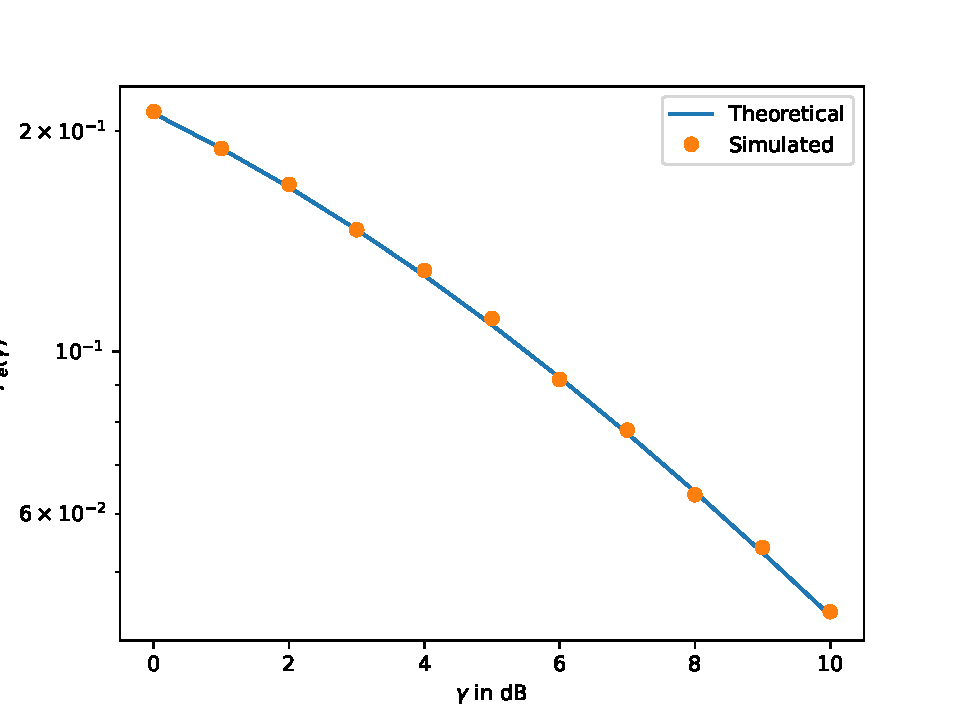
\includegraphics[scale=0.5]{../dig_com/Figs/6_6_4.pdf}      
\caption{The $P_e$ wrt $\gamma$ }
\label{fig:Pe_gamma1}
\end{figure}
\end{enumerate}
\section{Bivariate Random Variables:FSK}
\subsection{Two Dimensions}
Let 
\begin{equation}
\mbf{y} = A\mbf{x} + \mbf{n},
\end{equation}
where 
\begin{align}
x &\in \brak{\mbf{s}_0,\mbf{s}_1}, 
\mbf{s}_0 = 
\begin{pmatrix}
1 
\\
0
\end{pmatrix},
\mbf{s}_1 = 
\begin{pmatrix}
0 
\\
1
\end{pmatrix}
\\
\mbf{n} &= 
\begin{pmatrix}
n_1
\\
n_2
\end{pmatrix},
n_1,n_2 \sim \gauss{0}{1}.
\end{align}
\begin{enumerate}[label=\thesubsection.\arabic*,ref=\thesubsection.\arabic{figure}]
%%
\item
\label{ch5_fsk}
Plot 
%
\begin{equation}
\mbf{y}|\mbf{s}_0 \text{ and } \mbf{y}|\mbf{s}_1
\end{equation}
%
on the same graph using a scatter plot.\\
\solution The following python code plots the scatter plot when $\mbf{x} = \mbf{s}_0$ and $\mbf{x} = \mbf{s}_1$ in Fig. \ref{fig:scatter_2}
\begin{center}
\fbox{\parbox{10.5cm}{\href{https://github.com/AnushaJella/FWC1/blob/main/Digital-communications/codes/chapter7/7_1_1.py}{/codes/chapter7/7$\_$1$\_$1.py}}}
\end{center}
\begin{figure}
\centering
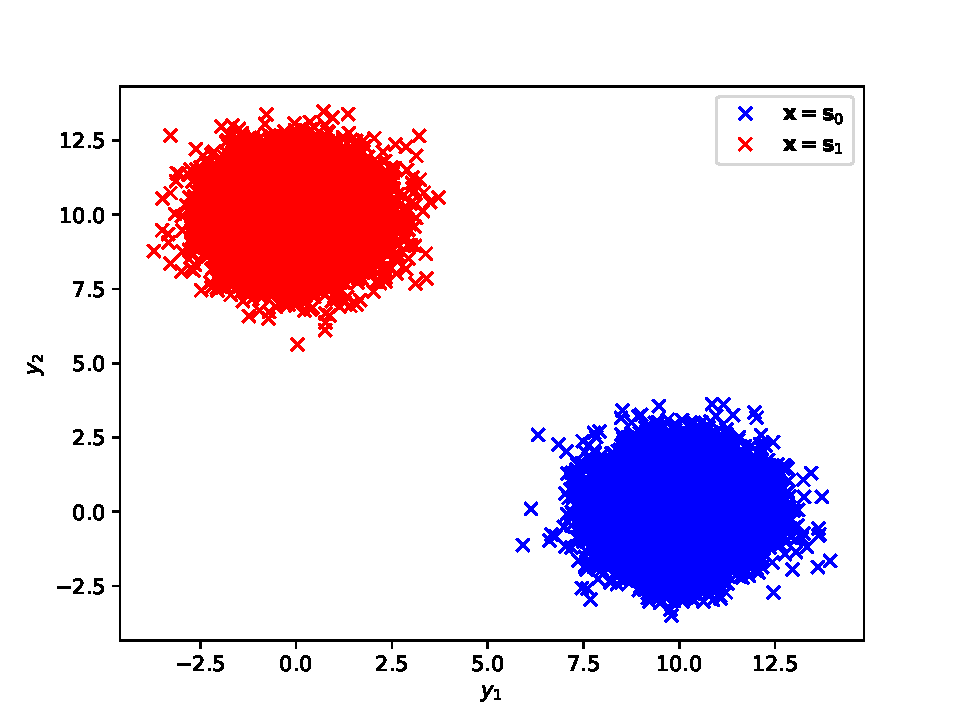
\includegraphics[scale=0.5]{../dig_com/Figs/y_scatter2.pdf}     
\caption{Y scatter plot }
\label{fig:scatter_2}
\end{figure}
\item
For the above problem, find a decision rule for detecting the symbols $\mbf{s}_0 $ and $\mbf{s}_1$.\\
\solution The multivariate Gaussian distribution is defined as
    %
    \begin{multline}
    \label{eq:multivariate}
    p_{\mathbf{x}}(x_1,\dots,x_k)
    =\frac{1}{\sqrt{\brak{2\pi}^k\abs{\mbf{\Sigma}}}}\exp\cbrak{-\frac{1}{2}\brak{\mathbf{x}-\mbf{\mu}}^T\mbf{\Sigma}^{-1}\brak{\mathbf{x}-\mbf{\mu}}}
    \end{multline}
    where $\mbf{\mu}$ is the mean vector, $\mbf{\Sigma} = E\sbrak{\brak{\mathbf{x}-\mbf{\mu}}\brak{\mathbf{x}-\mbf{\mu}}^T}$ is the covariance matrix and $\abs{\mbf{\Sigma}}$ is the determinant of $\mbf{\Sigma}$.
    For a bivariate gaussian distribution,
    {\small
    \begin{multline}
    \label{eq:bivariate}
    p(x,y)= \frac{1}{2\pi \sigma_x\sigma_y\sqrt{1-\rho^2}}\exp\lsbrak{-\frac{1}{2\brak{1-\rho^2}}}
    \\
    \times \rsbrak{\cbrak{\frac{\brak{x-\mu_x}^2}{\sigma_x^2}+\frac{\brak{y-\mu_y}^2}{\sigma_y^2}-\frac{2\rho\brak{x-\mu_x}\brak{y-\mu_y}}{\sigma_x\sigma_y}}}
    \end{multline}
    }
    %
    where
    %
    \begin{align}
\mbf{\mu}=\begin{pmatrix}
\mbf{\mu_x} \\
\mbf{\mu_y}
\end{pmatrix} , \mbf{\Sigma} = \begin{pmatrix}
\sigma_x^2 & \rho\sigma_x\sigma_y \\
    \rho\sigma_x\sigma_y & \sigma_y^2
\end{pmatrix} \\
\rho = \frac{E\sbrak{\brak{x - \mu_x}\brak{y-\mu_y}}}{\sigma_x\sigma_y}.
    %  
    \end{align}
        \begin{align}
        \mbf{y}|s_0 &= 
        \begin{pmatrix}
        A+n_1 \\
        n_2
        \end{pmatrix}\\
        \mbf{y}|s_1 &=  
        \begin{pmatrix}
        n_1 \\
        A+n_2
        \end{pmatrix}
        \end{align}
        Substituting these values in (\ref{eq:bivariate}),
        \begin{multline}
        \label{gauss_mutl_var1}
        p\brak{\mbf{y}|s_0} = \frac{1}{2\pi\sigma_{y_1}\sigma_{y_2}\sqrt{1-\rho_1^2}}\exp\lsbrak{-\frac{1}{2\brak{1-\rho_1^2}}}
        \\
        \times \rsbrak{\cbrak{\frac{\brak{y_1-A}^2}{\sigma_{y_1}^2}+\frac{\brak{y_2}^2}{\sigma_{y_2}^2}-\frac{2\rho_1\brak{y_1-A}\brak{y_2}}{\sigma_{y_1}\sigma_{y_2}}}}
        \end{multline}
        \begin{multline}
        \label{gauss_mutl_var2}
        p\brak{\mbf{y}|s_1} = \frac{1}{2\pi\sigma_{y_1}\sigma_{y_2}\sqrt{1-\rho_2^2}}\exp\lsbrak{-\frac{1}{2\brak{1-\rho_2^2}}}
        \\
        \times \rsbrak{\cbrak{\frac{\brak{y_1}^2}{\sigma_{y_1}^2}+\frac{\brak{y_2-A}^2}{\sigma_{y_2}^2}-\frac{2\rho_2\brak{y_1}\brak{y_2-A}}{\sigma_{y_1}\sigma_{y_2}}}}
        \end{multline}
        where,
        \begin{align}
        \label{rho_sig_val}
        \rho_1 = E[(y_1-A)(y_2)] &= E[n_1 n_2] = 0, \nonumber \\
        \rho_2 = E[(y_1)(y_2-A)] &= E[n_1 n_2] = 0, \nonumber \\
        \sigma_{y_1} = \sigma_{y_2} &= 1
        \end{align}
         For equiprobably symbols, the MAP criterion is defined as
        %
        \begin{align}
        \label{eq:map_bfsk_dec}
        p\brak{\vec{y}|s_0} &\dec{s_0}{s_1} p\brak{\vec{y}|s_1}
        \end{align}  
          Using (\ref{gauss_mutl_var1}) and (\ref{gauss_mutl_var2}) and substituting the values from (\ref{rho_sig_val}),  we get
        \begin{align}
        (y_1 -A)^2 + y_2^2 \dec{s_1}{s_0} y_1^2 + (y_2 - A)^2
        \end{align}
        On simplifying, we get the decision rule is
        \begin{align}
        \label{eq:decision_rule}
        y_1 \dec{s_0}{s_1} y_2
        \end{align}
\item
Plot 
\begin{equation} 
P_e = \pr{\hat{\mbf{x}} = \mbf{s}_1|\mbf{x} = \mbf{s}_0}
\end{equation}
with respect to the SNR from 0 to 10 dB.\\
\solution 
code available below and plot as shown in \ref{fig:Pe_snr2}
\begin{center}
\fbox{\parbox{10.5cm}{\href{https://github.com/AnushaJella/FWC1/blob/main/Digital-communications/codes/chapter7/7_1_3.py}{/codes/chapter7/7$\_$1$\_$3.py}}}
\end{center}
\begin{figure}
\centering
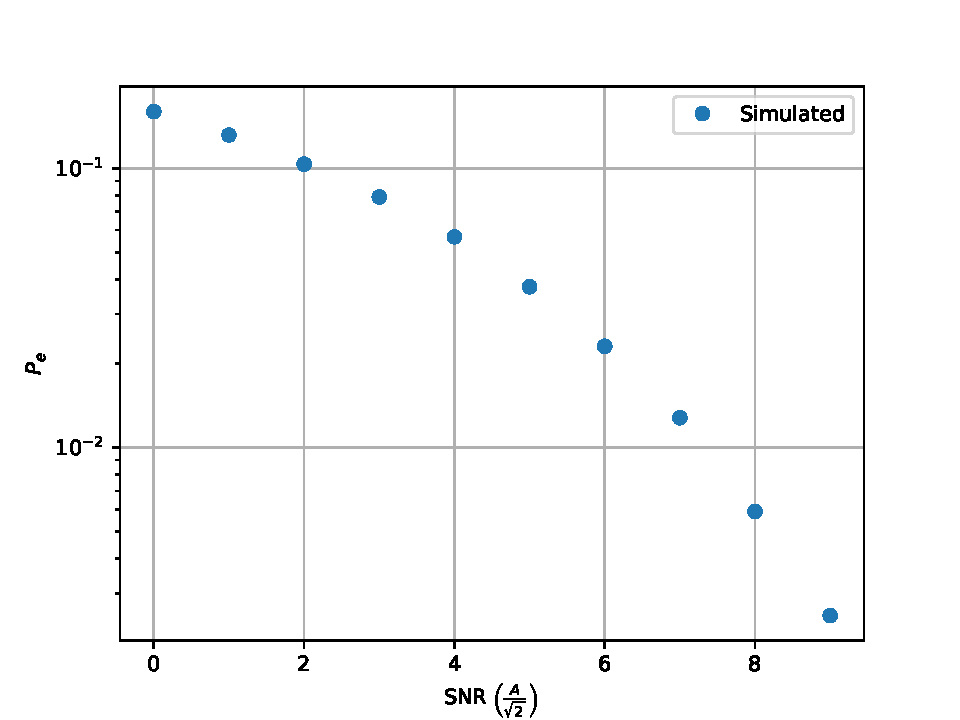
\includegraphics[scale=0.5]{../dig_com/Figs/err_snr_plot.pdf}       
\caption{Pe vs SNR }
\label{fig:Pe_snr2}
\end{figure}
\item
Obtain an expression for $P_e$. Verify this by comparing the theory and simulation plots on the same graph.\\
\solution 
    \begin{align}
    P_e = \pr{\hat{\mbf{x}} = \mbf{s}_1|\mbf{x} = \mbf{s}_0}
    \end{align}
    Given that $\mbf{s}_0$ was transmitted, the received signal is
    \begin{align}
    \mbf{y}|\mbf{s}_0 = \begin{pmatrix} A \\ 0 \end{pmatrix} + \begin{pmatrix} n_1 \\ n_2 \end{pmatrix}
    \end{align}
    From (\ref{eq:decision_rule}), the probability of error is given by 
    \begin{align}
    P_e &= \pr{y_1 < y_2 |\mbf{s}_0} = \pr{A+n_1 < n_2}\\
    &= \pr{n_2 - n_1 > A}
    \end{align}
    Note that $n_2 - n_1 \sim \gauss{0}{2}$. Thus,
    \begin{align}
    P_e &= \pr{\sqrt{2}w > A}\\
    \pr{w > \dfrac{A}{\sqrt{2}}}\\
    \Rightarrow P_e &= \qfunc{\frac{A}{\sqrt{2}}}
    \end{align}
    where $w \sim \gauss{0}{1}$. The following code plots the $P_e$ curve in Fig. (\ref{fig:Pe_snr3}).
    \begin{center}
\fbox{\parbox{10.5cm}{\href{https://github.com/AnushaJella/FWC1/blob/main/Digital-communications/codes/chapter7/7_1_4.py}{/codes/chapter7/7$\_$1$\_$4.py}}}
\end{center}
\begin{figure}
\centering
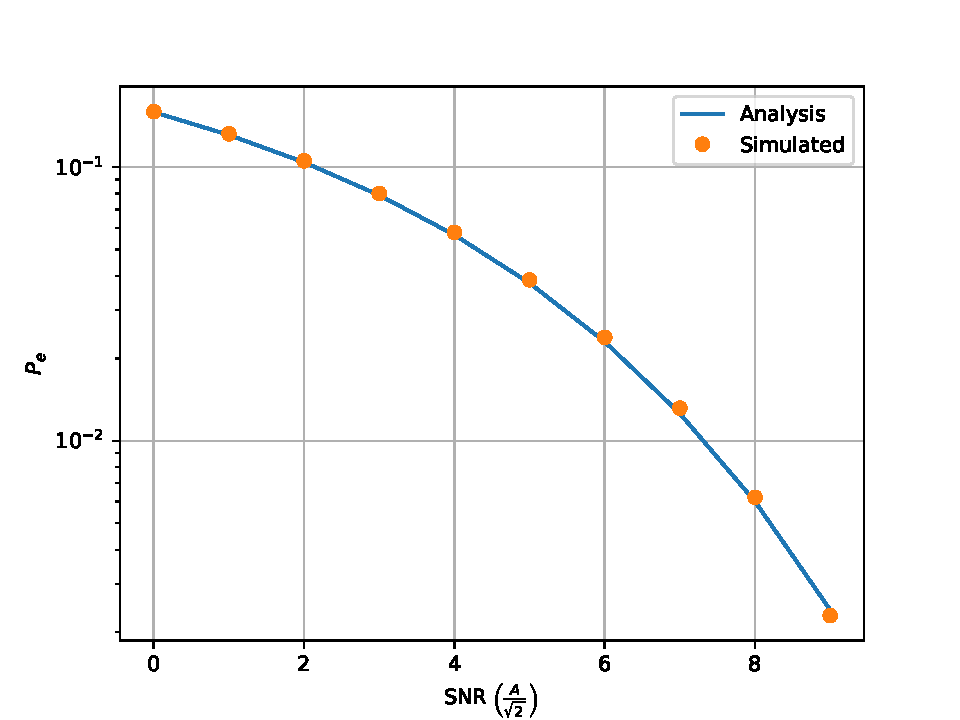
\includegraphics[scale=0.5]{../dig_com/Figs/Pe_snr_plot.pdf}       
\caption{Pe vs SNR on theory and simulation based }
\label{fig:Pe_snr3}
\end{figure}            
\end{enumerate}
%\end{enumerate}
\end{document}
